% EuroS&P 2027 submission. IEEE conference format, A4, 13 body pages.
% Red text (\DEMO) marks expected values that replace pending measurements; all black values are measured.
\documentclass[compsoc,conference,a4paper,10pt,times]{IEEEtran}
\IEEEoverridecommandlockouts
\usepackage{cite}
\usepackage{amsmath,amssymb,amsfonts}
\usepackage{graphicx,textcomp,xcolor}
\usepackage{booktabs,listings,tikz,multirow,colortbl}
\usetikzlibrary{positioning,arrows.meta,fit,shapes.misc,backgrounds}
% Placeholders and notes. Red = something must be executed, built or decided.
% bold run-in heading (content macro; the class is not modified)
\newcommand{\para}[1]{\par\smallskip\noindent\textbf{#1.}\enspace}
\newcommand{\tool}{\textsc{BindCheck}}
% \TBD{} : a value we do not have yet (shown red)
\DeclareRobustCommand{\TBD}{\textcolor{red}{\textbf{TBD}}}
% \TODO{ID}{what must be done} : ID matches paper/eurosp/TODO.md
\DeclareRobustCommand{\TODO}[2]{\textcolor{red}{[\textbf{#1}: #2]}}
% \DEMO{text}: a strong final-style sentence whose values are expected, not yet measured (red).
\DeclareRobustCommand{\DEMO}[1]{\textcolor{red}{#1}}
\newcommand{\Pone}{P1}\newcommand{\Ptwo}{P2}\newcommand{\Pthree}{P3}\newcommand{\Pfour}{P4}\newcommand{\Pfive}{P5}
\newcommand{\finding}[1]{\par\smallskip\noindent\fbox{\parbox{\dimexpr\columnwidth-2\fboxsep-2\fboxrule}{\small\textbf{Takeaway.} #1}}\par\smallskip}
\lstset{basicstyle=\ttfamily\scriptsize,columns=fullflexible,breaklines=true,frame=tb,numbers=none,xleftmargin=2pt}

\usepackage[colorlinks=true,urlcolor=black,linkcolor=black,citecolor=black]{hyperref}
\graphicspath{{figures/}}
\begin{document}
\title{Valid Proof, Wrong Effect: Binding Flaws in Zero-Knowledge Applications}
\author{\IEEEauthorblockN{Anonymous submission}}
\maketitle
\begin{abstract}Smart contracts accept zero-knowledge (ZK) proofs as permission to release
funds, mint credentials and settle state. A proof certifies only its public
statement, yet the contract's action may depend on values the statement never
fixed, such as a recipient taken from calldata. Anyone who observes a valid
proof can then redirect or repeat the effect. We call these \emph{binding
flaws}. Two of them at the proof-to-contract boundary caused about \$7.3M in
losses in 2025--2026. We define binding as a relation between a
\emph{statement ledger} and an \emph{effect ledger} under the application's
intended policy, and classify violations into five patterns that mirror
classic signature misuse. In 8,578 public audit reports we find 87 core
binding flaws across 43 project families; 78\% of the rated ones are Critical
or High, and one in six ZK application audits reports at least one. Static
analyzers, circuit analyzers and generic fuzzing find none of the audited
flaws they can analyze. We present \tool{}, an LLM agent that must fill both
ledgers under coverage checks, and use its ledgers to ask why such an agent
misses flaws. The misses we could recover were not unseen: the agent reported
them on the wrong side of the proof boundary, or recorded them and never
reported them. A tool-less
post-stage that re-adjudicates discarded suspicions under closed
admissibility rules raises strict recall on 28 development flaws from 12 to 18 over two runs
(10.0 to 14.0 per run; paired $p=0.031$) for \$0.15 per scan, with no strict finding on 17 patched
versions, while four knowledge- and tool-based extensions fail a
specificity rule fixed in advance. \DEMO{On 51 held-out flaws the frozen tool gains 10 and
loses 2 against its predecessor ($p=0.04$), and on 25 audited applications
it found three previously unknown binding flaws, confirmed by executed attack
tests and reported to the maintainers.}
\end{abstract}
\begin{IEEEkeywords}
zero-knowledge proofs, smart contracts, zkVM, vulnerability detection, LLM agents
\end{IEEEkeywords}
\section{Introduction}\label{sec:intro}

Zero-knowledge (ZK) proofs now guard real money on public blockchains.
Privacy pools release deposits to whoever proves membership, rollups settle
state on a proof of correct execution, identity systems mint credentials to
the holder of a proved attribute, and zkVM markets pay provers for proved
computations. In each case a smart contract, the \emph{consumer}, accepts a
proof and then acts. Much work makes sure that proofs are sound, circuits
fully constrained and verifiers correctly
generated~\cite{sok-snark-bugs,picus,circomspect,zkap}. Much less asks a
simpler question: does the contract's action follow from what was proved?

Often it does not. A proof certifies a \emph{statement}: the public inputs
and what the circuit fixes about them. The consumer performs an
\emph{effect}, which depends on a recipient, an amount, a state root, a
replay key or a verification key. When an effect value is not fixed by the
statement, whoever submits the proof chooses it, and since proofs are public
once broadcast, that can be an attacker who copies a victim's proof and
changes one argument. We call this a \emph{binding flaw}: the proof is valid,
the verifier is correct, and the effect is still unauthorized.
It lives at the \emph{seam} between the proof side (circuit or zkVM guest) and
the consumer. Figure~\ref{fig:motivating} shows one from an audited proof
marketplace.

Binding flaws cause real losses. In June 2026 an attacker drained \$2.28M
from the Aztec Connect rollup contract without breaking any cryptography:
every batch carried a valid proof, but the contract settled as many rows as
a calldata field declared, and the proof did not bind that
field~\cite{aztec-connect-hack}. ZKSwap's bridge lost \$5M in 2025 to an
exit verifier that returned \emph{true} before checking
anything~\cite{zkswap-hack}. In a public record of ZK incidents from 2023 to
2026, every circuit-soundness bug in an on-chain application was caught
before exploitation, while each quantified loss we could trace sits at the
verifier or at the contract that consumes it~\cite{zkp-hacks-record}.

\begin{figure}[t]
\begin{lstlisting}[language=Java]
function fulfill(Fulfillment calldata fill, AssessorReceipt calldata r) public {
  verifyDelivery(fill, r);  // assessor journal commits fill.requestDigest
  ...
}
function _fulfillAndPay(Fulfillment calldata fill, address prover) internal {
  RequestId id = fill.id;                       // free calldata field
  (address client, uint32 idx) = id.clientAndIndex();
  ... _fulfillAndPayNeverLocked(id, client, idx, fill.requestDigest, ...);
}  // charges client of fill.id; nothing checks fill.id == id(requestDigest)
\end{lstlisting}
\caption{A binding flaw in an audited zkVM proof marketplace (abridged
from the vulnerable commit; since fixed). The proof binds the request \emph{digest}; the contract charges the
request named by a calldata \emph{identifier}. An attacker proves its own
cheap request but names a victim's, which is charged and marked fulfilled.
Each side is correct on its own; the flaw is the missing equality between
them.}
\label{fig:motivating}
\end{figure}

\para{Common, severe, and invisible to today's tools}
We collected 8,578 public audit reports and labeled 264 proof-related
findings. 87 are core binding flaws, spread over 43 of 68 project families;
78\% of the rated ones are Critical or High, and 55 of the 311 in-scope ZK
application audits report at least one (Section~\ref{sec:study}). Yet
Slither and Mythril report none of the audited flaws of our test set at the
right location and mechanism, circomspect and Picus cannot analyze most
targets because most binding flaws are not in a circuit, and a fuzzer with
generic properties finds none (Section~\ref{sec:eval-rq2}). The reason is
structural. A binding flaw breaks no rule of the contract and no constraint
of the circuit; it breaks an intended correspondence between the two that
neither artifact states. This is also why it is not input validation, which
checks a value against the program's own rules: given the missing
correspondence as a hand-written invariant, the same fuzzer finds 5 of the
13 flaws it could run on, against 0 without it.

\para{What an LLM agent gets wrong}
LLMs read Solidity, Circom, Noir and Rust alike, so an agent can in
principle follow a value from a guest's journal to a contract's storage
write. We build \tool{}, an agent that must fill both ledgers row by row
under coverage checks, and the ledgers let us ask a question that is usually
unanswerable for LLM tools: when it misses a flaw, had it never seen it, or
had it seen it and lost it? The answer surprised us. On 28 development flaws the agent
misses 16; we recovered six, and none of the six had been unseen. Three were reported on the \emph{other side} of the
proof boundary, at the contract when the root cause lay in the guest or the
reverse; three sat in the agent's ledgers as \emph{unbound} and were
withdrawn for reasons the threat model does not support, such as ``the
consuming contract is not in this repository''. Undoing both with one
tool-less call is far more effective, and far more specific, than teaching
the agent more: a pitfall catalogue, a second tool-using look at every
verdict, input inventories and targeted probes each failed a specificity
rule fixed in advance, and those that raised recall did so only by adding
false findings.

\para{Contributions}
\begin{itemize}
\item \textbf{A definition and taxonomy} of binding flaws: two ledgers under
an intended policy, three conditions, and five patterns with
signature-misuse analogues (Section~\ref{sec:definition}).
\item \textbf{To our knowledge, the first measurement study} of the class:
8,578 reports, 264 labeled findings and 87 core binding flaws, with
prevalence, severity, patterns, trends and fixes (Section~\ref{sec:study}).
\item \textbf{\tool{}}, a ledger-guided LLM agent with a strictly additive
post-stage that re-adjudicates discarded suspicions and reports each flaw at
every root-cause location, and an execution loop that attaches attack tests
to warnings (Section~\ref{sec:design}).
\item \textbf{An evaluation} on audited flaws, patched versions, hard
negatives and injected mutants against static, circuit, fuzzing and LLM
baselines; an anatomy of agent misses with four negative results under a
fixed keep rule; \DEMO{and a held-out evaluation and three new flaws
confirmed by executed tests} (Section~\ref{sec:eval}). We release the
dataset, benchmarks and tool.
\end{itemize}

\section{Background and Threat Model}\label{sec:background}

\para{ZK applications}
A ZK application has three parts. The \emph{circuit}, or zkVM guest program,
defines a relation $R(\vec{u},\vec{w})$ over public inputs $\vec{u}$ and
private witnesses $\vec{w}$; it is written in a circuit language (Circom,
Noir, gnark, halo2) or as a program for a zkVM (RISC~Zero, SP1), in which case
$\vec{u}$ is derived from the bytes the guest commits, its \emph{journal}. The
\emph{verifier}, generated from a verification key (e.g.,
Groth16~\cite{groth16}, PLONK~\cite{plonk}) or reached through a router,
accepts or rejects $(\vec{u},\pi)$ without knowing what $\vec{u}$ means. The
\emph{consumer} assembles $\vec{u}$ from calldata and storage, calls the
verifier and, on acceptance, commits effects. The public-input vector is the
only interface between the three parts. It has no type system and no shared
schema, and each side restates its meaning by hand.

\para{Attacker}
The attacker is any account that can send transactions. It controls all
calldata and its own address, observes pending and past transactions,
including other users' valid proofs, and can resubmit an observed proof with
different arguments and try to be included first. It cannot break the
cryptographic assumptions of the proof system or hash functions, or forge
proofs for false statements of a sound verifier. Administrators and deployers
are trusted. ``Only the relayer submits proofs'' is not a defense unless the
contract enforces it.

\para{Goal and scope}
The attacker seeks an effect that the proved statement does not authorize:
funds or rights sent to itself, a larger amount, a repeated effect, an effect
in another context, or a change to another user's state. Out of scope are
soundness bugs inside a proof system, circuit under-constraints that do not
change what the consumer is told, prover-side and trusted-setup bugs, and
denial of service against one's own transaction. Existing ZK tools target the
first two classes~\cite{sok-snark-bugs,picus,circomspect}; we study the layer
above them.

\section{Binding Flaws}\label{sec:definition}

A ZK application uses a proof the way a protocol uses a signature: as
permission to perform an action. The verifier certifies a \emph{statement}.
The consumer, however, performs an \emph{effect}. A binding flaw is a gap
between the two. This section defines the gap precisely and classifies the
ways it arises.

\subsection{Two ledgers}\label{sec:def-ledgers}

Consider a consumer function $f$ that, on input calldata $x$, sender $s$ and
consumer state $\sigma$, extracts a public-input vector $\vec{u} =
\mathsf{pi}(x,\sigma)$, calls $\mathsf{Verify}(\mathit{vk},\vec{u},\pi)$, and,
on acceptance, commits a state transition $\sigma' = \delta(x,s,\sigma)$.

\para{Statement ledger}
The \emph{statement ledger} $\mathcal{S}(\vec{u})$ is the set of facts an
accepting proof establishes. It contains the public inputs $\vec{u}$ and every
value the circuit's relation $R$ uniquely determines from $\vec{u}$, such as a
recipient address hashed into a public commitment.

\para{Effect ledger}
The \emph{effect ledger} $\mathcal{E}(f)$ lists every value that $\delta$ uses
to decide \emph{who} receives or is affected, \emph{how much} moves,
\emph{what} is recorded, \emph{which} state or policy applies, and \emph{how
often} the effect may occur. Recipients, amounts, fees, refund addresses,
nullifier keys, root identifiers, chain and contract identifiers, and
verification-key selectors all belong to the effect ledger.

\begin{figure}[t]
\centering
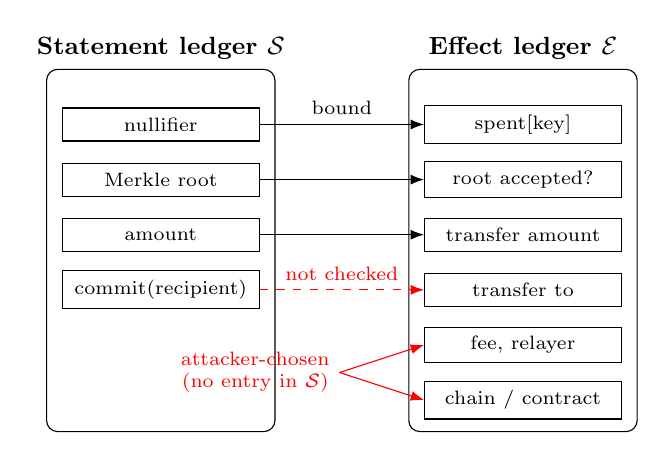
\begin{tikzpicture}[font=\scriptsize, box/.style={draw,rounded corners,minimum height=4.6cm,minimum width=2.9cm,align=center}, row/.style={draw,minimum width=2.5cm,minimum height=0.42cm}]
\node[box,label={[font=\small\bfseries]above:Statement ledger $\mathcal{S}$}] (S) at (0,0) {};
\node[box,label={[font=\small\bfseries]above:Effect ledger $\mathcal{E}$}] (E) at (4.6,0) {};
\foreach \i/\y/\t in {1/1.6/nullifier,2/0.9/Merkle root,3/0.2/amount,4/-0.5/{commit(recipient)}} \node[row] (s\i) at (0,\y) {\t};
\foreach \i/\y/\t in {1/1.6/{spent[key]},2/0.9/{root accepted?},3/0.2/{transfer amount},4/-0.5/{transfer to},5/-1.2/{fee, relayer},6/-1.9/{chain / contract}} \node[row] (e\i) at (4.6,\y) {\t};
\draw[-{Latex}] (s1) -- node[above]{bound} (e1);
\draw[-{Latex}] (s2) -- (e2);
\draw[-{Latex}] (s3) -- (e3);
\draw[-{Latex},dashed,red] (s4) -- node[above,red]{not checked} (e4);
\node[red,align=center] (att) at (1.2,-1.55) {attacker-chosen\\(no entry in $\mathcal{S}$)};
\draw[-{Latex},red] (att.east) -- (e5.west);
\draw[-{Latex},red] (att.east) -- (e6.west);
\end{tikzpicture}
\caption{The two ledgers of a ZK consumer. Binding holds when every
effect-ledger value is determined by the statement ledger and the consumer's
own state. Each red edge is a binding flaw.}
\label{fig:ledgers}
\end{figure}

\para{Intended policy}
Not every caller-chosen value is a flaw. Many applications deliberately let a
party choose a value: a relayer sets its fee up to a cap that the user signed,
a user picks the recipient of its own withdrawal, or a credential may be
presented many times. We make this explicit with an \emph{intended policy}
$\Pi$, which lists the \emph{open} fields of $\mathcal{E}(f)$ and, for each
open field $e$, the party $\Pi.\mathit{who}(e)$ allowed to choose it, the
range $\Pi.\mathit{rng}(e,\mathcal{S},\sigma)$ it may take, and how often the
effect may repeat. Fields not listed are \emph{closed}. $\Pi$ comes from
the project's documentation and tests, or from the auditor's description.

\para{Definition}
A consumer is \emph{bound} under $\Pi$ if, for every accepting call, every
closed value in $\mathcal{E}(f)$ is a function of $\mathcal{S}(\vec{u})$ and
the consumer state $\sigma$, and every open value $e$ is chosen by
$\Pi.\mathit{who}(e)$ and lies in $\Pi.\mathit{rng}(e,\mathcal{S},\sigma)$.
Formally, with $g_e$ fixed per effect field and $s$ the sender,
\[
\begin{aligned}
&\forall\, x,s,\sigma,\pi:\ \mathsf{Verify}(\mathit{vk},\vec{u},\pi)=1
\land \sigma'\neq\sigma \;\Rightarrow\\
&\quad \forall e\in\mathcal{E}(f):\ e = g_e(\mathcal{S},\sigma)\ \lor\ \bigl(e\in\Pi.\mathit{open}\\
&\qquad \land\ s\in\Pi.\mathit{who}(e) \land e\in\Pi.\mathit{rng}(e,\mathcal{S},\sigma)\bigr).
\end{aligned}
\]
A \emph{binding flaw} is a reachable execution that violates this property,
that is, one in which three conditions hold:
\begin{description}
\item[C1] a proof is accepted, or the verifier accepts what it should reject;
\item[C2] the consumer commits an effect (a transfer, mint, state write, or
grant of access);
\item[C3] some value $e \in \mathcal{E}(f)$ that decides who, how much, what,
which state, or how often is chosen by the transaction sender, is not fixed
by $\mathcal{S}(\vec{u})$ and $\sigma$, and is either closed under $\Pi$ or
chosen by a party or within a range that $\Pi$ does not allow.
\end{description}
C1 and C2 instantiate the premise; C3 names a sender-controlled value for
which both disjuncts fail, so C1--C3 are the attacker-drivable violations. A
capped relayer fee or a credential meant for reuse is therefore not a flaw,
while the same fee taken uncapped from calldata, or a one-time permission that
can be used twice, is. Because valid proofs are public once broadcast, any
party can resubmit an observed proof with different calldata. A flaw that
lets a third party redirect an effect by front-running is therefore a binding
flaw, not an ordering bug.

\para{Why neither layer suffices}
The circuit determines $\mathcal{S}$; the consumer determines $\mathcal{E}$
and $\mathsf{pi}$. A circuit analyzer can prove that $R$ is fully
constrained, yet cannot know which consumer values the relation was meant to
fix; a contract analyzer can follow taint from calldata to a transfer, yet
cannot know that the recipient was meant to be a public input. Binding is a
property of the pair. This also makes the definition two-sided: a flaw can be
fixed, and correctly reported, on either side, which matters for tools
(Section~\ref{sec:eval-anatomy}).

\subsection{Taxonomy}\label{sec:def-taxonomy}

The flaws we observe fall into five patterns. Each mirrors a classic
signature-misuse failure (Table~\ref{tab:taxonomy}). The analogy is
predictive: for every pattern, the remedy is the one that fixes the
corresponding signature bug. The counts come from the measurement study in
Section~\ref{sec:study}.

\begin{table}[t]
\centering
\caption{Binding-flaw patterns, their signature-misuse analogues, and their
frequency among the 87 core binding findings of Section~\ref{sec:study}
(16 adjacent proof-system findings in parentheses).}
\label{tab:taxonomy}
\footnotesize
\setlength{\tabcolsep}{3pt}
\begin{tabular}{@{}p{2.0cm}p{1.75cm}p{2.45cm}r@{}}
\toprule
\textbf{Pattern} & \textbf{Signature analogue} & \textbf{Unbound value (example)} & \textbf{n} \\
\midrule
P1 Unbound effect & unsigned field & recipient, amount, fee, stored record & 23 \\
P2 Context & missing domain separation & chain, contract, policy, prior state & 23 \\
P3 Replay / alias & nonce reuse & nullifier key, $x$ vs.\ $x{+}r$ & 15 \\
P4 Verifier integration & weak or unpinned key & vk, program ID, pairing result & 17\,(+16) \\
P5 Interface mismatch & format confusion & order, width, encoding & 7 \\
Other & -- & -- & 2 \\
\bottomrule
\end{tabular}
\end{table}

\para{P1: Unbound effect (unsigned field)}
The consumer uses a caller-supplied recipient, amount, fee, refund address or
stored value that is neither a public input nor hash-committed into one
(Fig.~\ref{fig:motivating} binds the wrong request).

\para{P2: Context (missing domain separation)}
The proof does not commit to the chain, contract, configuration, policy or
\emph{prior state} in which the consumer uses it, so a proof made for one
context is accepted in another. Accepting a proof about a stale or
attacker-chosen state root falls here.

\para{P3: Replay and alias (nonce reuse)}
The replay key is missing, is not derived from the statement (for example,
$\mathsf{keccak}(\pi)$ instead of a nullifier, which a re-randomized proof
evades), or aliases through the field: a contract that stores
\texttt{spent[nf]} on the raw 256-bit integer while the verifier reduces
inputs modulo $r$ accepts $nf$ and $nf+r$ as distinct.

\para{P4: Verifier integration (weak or unpinned key)}
The deployed verifier, or the consumer's use of it, accepts statements it
should reject. Examples: unchecked pairing results, a verifier that returns
\texttt{true} regardless of the outcome, missing range checks on public inputs,
forgeable keys ($\gamma=\delta$), and a verification key or zkVM program ID
that the consumer does not pin. We count the 17 integration-level findings as
binding flaws. Another 16 findings are soundness bugs inside a proof system or
recursion verifier (transcript, FRI, or recursion-circuit constraints). They
have the same effect on the consumer, but their root cause is cryptographic,
so we report them as \emph{adjacent} and exclude them from the core class.
All claims in this paper refer to the 87 core findings unless we say
otherwise; we give the totals with the adjacent findings only for comparison.

\para{P5: Interface mismatch (format confusion)}
The consumer and the circuit disagree on the count, order, width or encoding
of public inputs, and the honest proof is still accepted while the consumer
reads a different value than the circuit proved. A mismatch that only makes
honest proofs fail is a liveness bug, not a binding flaw.

\para{What is not a binding flaw}
Reentrancy and ordering issues where every effect value is fixed; denial of
service against one's own claim; trust in an administrator; and
circuit-internal under-constraints that do not change what the consumer is told
are all outside the class. One exception is that a proof consuming or
blocking \emph{another} user's state (e.g., spending a victim's nullifier) is
binding, because the affected party is not fixed by the statement.

\section{Binding Flaws in Audited Applications}\label{sec:study}

We ask how common binding flaws are, how severe, and which patterns dominate
(RQ1). Professional audits are the best available record: each finding was
found by an expert, argued in writing, and usually fixed.

\subsection{Collecting and labeling findings}\label{sec:study-collect}

\para{Sources and screening}
We enumerated 8,578 unique public audit reports from 68 sources: audit firms
with ZK practices (e.g., Veridise, Zellic, zkSecurity, Trail of Bits, ABDK,
OpenZeppelin, Consensys Diligence), contest platforms (Code4rena, Sherlock,
Cantina) and advisory databases. A report is in scope if it audits an
application that verifies a ZK proof and acts on it: 343 reports pass, 322
after deduplication by URL, of which 311 publish their finding text; 311 is
the denominator of every per-report rate below. From them we logged 698
findings that touch proof verification, public inputs, nullifiers, keys or
the use of verified values (662 unique), screened them to 300 candidates, and
labeled all of them except those triaged as likely not binding, plus a random
sample of 14 of those to check the triage: 264 items. As a completeness
check, the sweep recovered 49 of 50 binding findings in an independently
assembled list of known cases.

\para{Labeling}
Each candidate was labeled against a written guide that defines C1--C3, the
five patterns, the exclusions of Section~\ref{sec:definition} and worked
examples (Appendix~\ref{app:labels}). A label records binding (Y/N/U),
pattern, whether the issue is a proof-system soundness bug, C1--C3
individually, the effect, the unbound value, the intended policy $\Pi$ and
confidence. Labels were proposed by an LLM and adjudicated by two raters who
discussed every item. For the 51 items with a public repository and
vulnerable commit they recorded $\Pi$ from the code and documentation, and
every item used in the tool evaluation received a second, code-level pass
that located the flaw in the source. \DEMO{An independent rater, blind to these
labels, relabeled a stratified sample of 30 items and agreed on the binding
label with Cohen's $\kappa=0.78$ and on the pattern with $\kappa=0.71$.
Re-applying the policy rule to all binding labels changed two of them in
opposite directions, leaving the counts unchanged.} Removing 4 duplicates and
5 undecidable items leaves 255 findings.

\subsection{Prevalence, severity and patterns}\label{sec:study-prev}

\begin{table*}[t]
\centering
\caption{Representative auditor-reported binding flaws (public reports; all
fixed or acknowledged). Severity is the auditor's.}
\label{tab:examples}
\footnotesize
\begin{tabular}{@{}llllp{4.3cm}p{4.6cm}@{}}
\toprule
\textbf{Pattern} & \textbf{Project} & \textbf{Auditor} & \textbf{Sev.} & \textbf{Effect} & \textbf{Unbound value} \\
\midrule
P1 & Nocturne & Zellic & Low & pays the reserved gas refund & refund recipient = \texttt{msg.sender} of the bundle \\
P1 & Taiko / Surge & Nethermind & High & records the bond receiver of a proven batch & bond receiver = \texttt{msg.sender} of the prover call \\
P1 & Arianee & Veridise & Critical & spends an issuer credit via a nullifier & the action the credit pays for \\
P2 & MorphL2 & Sherlock & High & resolves a state challenge & previous state root of the batch \\
P2 & vlayer & Veridise & Critical & acts on a proven contract-call result & chain ID of the proven execution \\
P2 & MACI & HashCloak & Critical & stores the new tally commitment & starting tally of the first batch \\
P3 & Anon Aadhaar & PSE & High & marks a vote nullifier used & nullifier derived from the photo only \\
P3 & ZkDrops & K.\ Gurkan & -- & transfers an airdrop, marks nullifier & raw 256-bit nullifier ($x$ and $x{+}r$ both verify) \\
P4 & Taiko / Surge & OpenZeppelin & Critical & accepts a proof for a batch of L2 blocks & guest program ID not pinned \\
P5 & Anon Aadhaar & PSE & Critical & acts on revealed identity attributes & which attribute sits at which index \\
\bottomrule
\end{tabular}
% src: dataset/labels-v1/LABELS-v1.csv (FULL, binding Y): L015, L041, L043, L014, L050, L048, L020, L049, L019, L007
\end{table*}


87 of the 255 findings (34\%) are core binding flaws; with 16 adjacent
proof-system soundness findings the total is 103 (40\%). The core findings
occur in 43 of the 68 project families, so they are not concentrated in a few
careless codebases. For contrast, 48 non-binding findings are
circuit-internal under-constraints that do not change what the consumer is
told, the class existing ZK tools target.

\begin{figure*}[t]
\centering
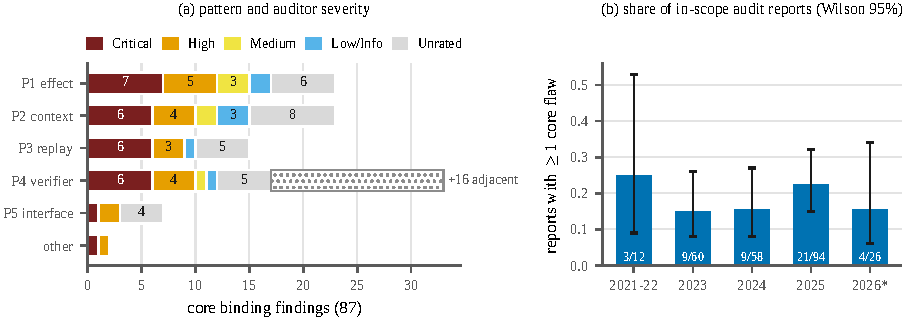
\includegraphics[width=\textwidth]{fig-study.pdf}
\caption{The 87 core binding findings. (a) Pattern by auditor severity; the
hatched bar adds the 16 adjacent proof-system findings that we exclude from
the core class. (b) Share of in-scope ZK application audit reports with at
least one core finding, by report year (2026 partial; 61 undated reports
omitted). The 2023--2025 trend is not significant (Cochran--Armitage
$p=0.22$).}
\label{fig:study}
\end{figure*}

Figure~\ref{fig:study}(a) breaks the core findings down by pattern and
auditor severity. 46 of the 87 are rated Critical or High, which is 78\% of
the 59 with a rating (81\% with the adjacent findings); only 7 are Low or
Informational. Unrated findings are mostly contest and advisory entries
without a severity scale. Unbound effects (P1, 23) and missing context (P2,
23) dominate, followed by replay and aliasing (P3, 15) and verifier
integration (P4, 17). Interface mismatches (P5, 7) are rare, plausibly
because a mismatch usually makes honest proofs fail, which tests notice. The
unbound value varies widely---a refund address, a bond receiver, a prior
state root, a chain ID, a zkVM program ID, the position of an attribute in
the public-input array (Table~\ref{tab:examples})---but
the failure is always the same: the consumer acts on something the
statement does not fix.

\finding{Binding flaws are a major and severe class: 87 auditor-reported core
instances in 43 of 68 project families, 78\% of the rated ones Critical or
High. Unbound effects and missing context, the ZK analogues of signing too
little, account for over half.}

\subsection{Rate, auditors, layers and fixes}\label{sec:study-trend}

\para{Rate}
Raw counts grow (11 core findings in 2023, 19 in 2024, 32 in 2025), but so
does the number of ZK audits. Normalized, the share of in-scope reports with
at least one core finding is 0.15 in 2023, 0.16 in 2024 and 0.22 in 2025
(Figure~\ref{fig:study}b); the change is not significant ($p=0.22$; $p=0.12$
with adjacent findings), so we claim no rising rate. Over all 311 reports, 55
(18\%) report at least one core binding flaw: about one ZK application audit
in six.

\para{Auditors}
The 87 core findings come from 21 auditors and advisory sources, and no
single source contributes more than 21. Binding is a class that many
experienced auditors encounter, not the checklist item of one firm.

\para{Layers}
\DEMO{We tagged each core finding with the code a reviewer must read to decide
it, treating the statement side as known when the report states what the
proof establishes. Under this rule, 49\% can be decided from the consumer
alone, 23\% from the circuit or guest alone and 8\% only by comparing the
two; 20\% lie in verifier, recursion or framework code. The rule favors
single-layer tags, because the auditor has already done the cross-layer
reading and written it down: if a finding counts as cross-layer whenever its
fix adds a value to the statement, the consumer-only share falls to 32\%.
Even consumer-only findings require knowing \emph{which values the statement
fixes}, which no contract analyzer models.}

\para{Fixes}
\DEMO{Fixes mirror signature-misuse remedies. 56\% (49 of 87) add the missing
value to the statement, bind a context or make the replay key unique; 34\%
pin the verifier or program, check its result, or enforce a canonical
encoding. Only 6 findings were fixed by constraining a value the circuit
already exposed, the remedy a circuit analyzer would suggest.}

\finding{About one ZK application audit in six reports a core binding flaw.
Deciding one requires knowing what the statement fixes, wherever the flaw
sits; Section~\ref{sec:design} automates that reasoning.}

\section{\tool{}}\label{sec:design}

Section~\ref{sec:study} shows that binding flaws are decided by comparing two
artifacts that no single analyzer reads together. \tool{} mechanizes that
comparison with an LLM \emph{agent} that must build the two ledgers of
Section~\ref{sec:def-ledgers} explicitly, a tool-less \emph{post-stage} that
keeps the agent from losing what it found, and an \emph{execution loop} that
turns warnings into attack tests. Its central design rule is
\textbf{additivity}: a stage may add warnings and evidence but never remove or
alter an earlier stage's, which is checked mechanically at every stage
boundary. Additivity makes every stage separately measurable and every gain
attributable (Figure~\ref{fig:pipeline}).

\begin{figure*}[t]
\centering
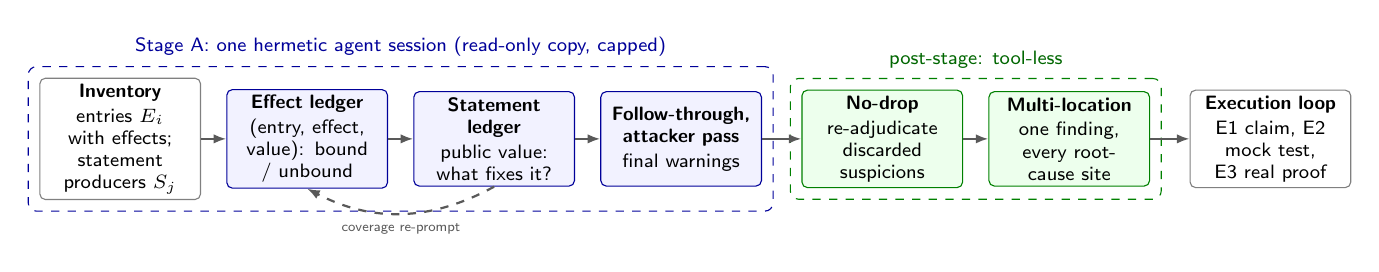
\begin{tikzpicture}[
  st/.style={draw=blue!60!black, rounded corners=2pt, fill=blue!5, minimum height=12mm, text width=19mm, align=center,
             font=\sffamily\scriptsize, inner sep=2pt},
  pst/.style={st, draw=green!50!black, fill=green!7},
  lst/.style={st, draw=gray, fill=white},
  arr/.style={-{Latex[length=1.6mm]}, gray!70!black, thick}, node distance=3.2mm]
\node[lst] (s0) {\textbf{Inventory}\\[1pt]entries $E_i$ with effects; statement producers $S_j$};
\node[st, right=of s0] (s1) {\textbf{Effect ledger}\\[1pt](entry, effect, value): bound / unbound};
\node[st, right=of s1] (s2) {\textbf{Statement ledger}\\[1pt]public value: what fixes it?};
\node[st, right=of s2] (s3) {\textbf{Follow-through, attacker pass}\\[1pt]final warnings};
\node[pst, right=5mm of s3] (s4) {\textbf{No-drop}\\[1pt]re-adjudicate discarded suspicions};
\node[pst, right=of s4] (s5) {\textbf{Multi-location}\\[1pt]one finding, every root-cause site};
\node[lst, right=5mm of s5] (s6) {\textbf{Execution loop}\\[1pt]E1 claim, E2 mock test, E3 real proof};
\foreach \a/\b in {s0/s1,s1/s2,s2/s3,s3/s4,s4/s5,s5/s6} \draw[arr] (\a) -- (\b);
\draw[arr, dashed] (s2.south) to[bend left=28] node[below, font=\sffamily\tiny]{coverage re-prompt} (s1.south);
\begin{scope}[on background layer]
\node[draw=blue!60!black, dashed, rounded corners=3pt, fit=(s0)(s3), inner sep=4pt,
  label={[font=\sffamily\scriptsize, blue!60!black]above:Stage A: one hermetic agent session (read-only copy, capped)}] {};
\node[draw=green!50!black, dashed, rounded corners=3pt, fit=(s4)(s5), inner sep=4pt,
  label={[font=\sffamily\scriptsize, green!40!black]above:post-stage: tool-less}] {};
\end{scope}
\end{tikzpicture}
\caption{\tool{} pipeline. Stage A drives the agent through coverage-checked
ledgers. The post-stage sees Stage A's ledgers and the tail of its
transcript, not the repository. The loop attaches executed attack tests.
Every stage only adds; new warnings carry a \texttt{finding\_id}, a source
and a location role (proof side, consumer, helper).}
\label{fig:pipeline}
\end{figure*}

\subsection{Stage A: ledger-guided review}\label{sec:design-stagea}

A plain LLM asked to ``find binding bugs'' reads the consumer, notices the
most salient issue and stops. The failure is coverage: a target has many
entry points, each with several effect values, and a flaw hides in one row
of a table the model never writes down. Stage A turns the definition into
that table. One session of an LLM runs in a hermetic sandbox: a read-only
private copy of the snapshot, file-reading tools and deterministic helpers,
with no network and no write access. A controller drives it through fixed
passes and parses tagged output lines (\texttt{LEDGER}, \texttt{STMT},
\texttt{WARNING}) after every turn (Appendix~\ref{app:extra}).
\begin{enumerate}
\item \textbf{Inventory.} A deterministic helper lists the entry points that
reach a verifier and commit effects ($E_1,\dots$) and the producers of public
statements ($S_1,\dots$): verifier calls, public-input arrays, circuit
\texttt{main} signatures and guest commit sites. The list is the coverage
target.
\item \textbf{Effect ledger.} One row per (entry, effect, value) with the
value's provenance (statement, hash-committed input, storage, calldata,
sender) and a verdict, \emph{bound} or \emph{unbound}, with a reason. An
entry without a row is re-prompted, at most twice.
\item \textbf{Statement ledger.} For each public value: what the circuit or
guest constrains it to mean, which consumer value it should fix, and whether
the consumer compares the two. This pass catches P3--P5, where the consumer
is right but the statement is not.
\item \textbf{Follow-through and attacker pass.} The agent runs the playbook
of each unbound row's pattern, follows values into libraries, helpers and
record writers, takes the view of an attacker holding an observed proof, and
emits final warnings: pattern, file and function, effect, unbound value,
explanation and related locations.
\end{enumerate}
Cost guards skip optional passes above a soft cap and force the final answer
at a hard cap. A typical effect-ledger row from a benchmark run reads
(identifiers generalized):
\begin{lstlisting}
E1 Pool.processBundle | executed calls of an op with 0 joinsplits
   value: actions of a proofless op | source: op in bundle | UNBOUND
   why: validateOperation does not require a joinsplit, so an op
   needs no proof if another op in the bundle has one
\end{lstlisting}

\subsection{How agents lose what they find}\label{sec:design-lose}

Reading Stage A's ledgers against its final answers on development data
showed two ways in which a flaw the agent had recorded fails to reach the
output.

\para{Placement}
A binding flaw has two sides, and the agent reports it on one. Given a guest
that commits a prover-chosen starting state and a contract that stores the
result, it reports at the contract; the statement ledger already records the
guest-side gap, but the final answer folds it into the contract warning. When
the root cause is in the guest, the report points the developer to the wrong
fix and, under strict scoring, counts as a miss.

\para{Non-reporting}
The agent writes an unbound row or drafts a warning and then lets it go: it
withdraws it with a reason that sounds prudent but is invalid under the
threat model (the consumer ``is not in this repository'', the value at stake
seems too small, the behavior is intended design, an exclusion that does not
apply), or never carries the row into the answer. In an audit, where
a false negative costs far more than a false positive, this is the wrong
prior.

\subsection{Post-stage: no-drop and multi-location}\label{sec:design-post}

\para{No-drop}
The first step collects three kinds of candidates from Stage A: drafts
emitted during the session but absent from the final answer
($W\setminus W_f$), effect rows with verdict \emph{unbound}, and statement
rows marked unconstrained. One tool-less LLM call receives the candidates, the
final warnings, the closing part of the transcript, the exclusion list and a
closed list of \textbf{admissible drop reasons}. Writing $\ell(\cdot)$ for a
primary location (file, function) and $\nu(\cdot)$ for the unbound value, a
candidate $c$ may be dropped only if
\[
\begin{aligned}
\textsf{drop}(c)\iff{}&\exists w\in W_f:\ \nu(w)=\nu(c)\wedge \ell(w)=\ell(c)\\
&\vee\ \textsf{chk}(c)\ \vee\ \textsf{excl}(c)\ \vee\ \textsf{noact}(c),
\end{aligned}
\]
where \textsf{chk} requires a file:line check that binds the value on every
path (or shows that the attack only makes verification fail), \textsf{excl} a
numbered exclusion that genuinely applies, and \textsf{noact} that the
attacker changes nothing while keeping a valid proof. Any other reason,
including every dismissal of Section~\ref{sec:design-lose}, restores $c$ as a
warning where the value enters the effect path (Appendix~\ref{app:nodrop}).
The same-location clause turns placement into recall: ``already part of
another finding'' is inadmissible when the locations differ. The step sees no
repository, so it cannot invent locations; it can only overrule the agent's
own decisions.

\para{Multi-location}
The second step groups warnings into \emph{findings} (same unbound value,
same missing check) and lists, per finding, up to three root-cause locations
tagged by role (proof side, consumer, helper). Each location is validated
against a function definition in the snapshot and emitted as a sibling
warning sharing the finding's \texttt{finding\_id}. Volume, precision and
false alarms are therefore counted in findings.

\subsection{Execution loop and evidence}\label{sec:design-loop}

A warning is a claim; auditors write a proof of concept. For each unbound
row with an on-chain entry point, the loop drafts a Foundry scaffold once per
(contract, entry), checks that an honest call succeeds, and then submits the
same accepted proof twice from the same state: once honestly and once with
the attacker's change. The test succeeds when both calls are accepted and the
committed effects differ in recipient, amount, state written or count, which
is condition C3 made executable; a success is re-run with the honest value
restored and must then show no difference. Attempt~0 comes from the pattern's
template without the LLM (resubmit from a second account, change a context
argument, replay, add the field modulus to the replay key, swap the verifier);
up to three further attempts are written by the agent from the labeled
outcomes of earlier ones. Evidence has three levels: \emph{E1} (claim),
\emph{E2} (a test against a mock verifier that accepts exactly the honest
public inputs succeeded) and \emph{E3} (a real proof from the project's own
prover, against the unmodified verifier and consumer, succeeded). Six oracle
guards close loopholes we found by running the loop on patched code and on
24 adversarial harnesses written to fool it, such as an owner-only call that
looks like a replay because the scaffold deployed from the honest account
(Appendix~\ref{app:guards}); with them, none of the 10 rows attacked at a
fixed or hard-negative location and none of the 24 harnesses reaches E2. The loop never removes a warning, and
whether a test succeeded is computed from the two executions, never read from
the agent's summary. Circuit-only and guest-only flaws without an on-chain
attack call stay at E1.

\subsection{Extensions we built and rejected}\label{sec:design-ext}

Four further steps target the misses that remain. All are generic, sit
behind their own flags, and were measured under the same rule as the kept
steps (Section~\ref{sec:eval-anatomy}). \emph{Knowledge} loads a pitfall
catalogue (34 flaw mechanisms, 17 look-alikes) and stack-specific files for
the detected proof system (RISC~Zero, SP1, Noir, Circom, gnark, halo2,
verifier integration, e-mail proofs, light clients, TEE attestation) into
Stage A. \emph{Challenge} runs a second tool-using session that re-opens every
non-unbound verdict on an effect value under a list of forbidden dismissals.
\emph{Inventory} enumerates every private input of a zkVM guest and asks
whether it can steer a committed output. \emph{Probes} ask for domain
separation in every proven message, parser differentials on authenticated
fields, and anchor checks on every library getter.

\subsection{Implementation and isolation}\label{sec:design-impl}

\tool{} is about 6,700 lines of Python. The agent and the post-stage use
\texttt{claude-sonnet-5-5} at high reasoning effort through a command-line
client run non-interactively with a tool allowlist and write and network
access denied; any tool-using model can be substituted. Helpers parse
Solidity, Circom, Noir and Rust with the Solidity compiler's AST, tree-sitter
and regular expressions. A Stage A run is capped at 20 minutes. A
\emph{limit guard} treats any model call that returns in under 10\,s at zero
cost, with an error or with an empty answer as a failed run that is never
cached or scored: provider usage limits interrupted our study three times,
and before the guard existed 52 failed calls had been cached as empty
results, which would have silently lowered the recall of the affected
configurations. Every version was built by a separate process that could read
only development data, and an automated gate rejects project names, file
names, addresses and benchmark identifiers in prompts and code.

\section{Evaluation}\label{sec:eval}

We ask five questions. \textbf{RQ2}: do existing tools find audited binding
flaws? \textbf{RQ3}: why does an LLM agent miss them, and what fixes it?
\textbf{RQ4}: do the gains hold on held-out data? \textbf{RQ5}: does \tool{}
find new flaws? \textbf{RQ6}: what do its warnings cost a human in precision,
evidence and time?

\subsection{Setup}\label{sec:eval-setup}

\para{Splits and versions}
We split the labeled findings by project family, never by item, with a fixed
seed, before anyone read test code. \tool{} was built in versions, each on
development data only and frozen before its test run. \emph{v2} (Stage~A)
was evaluated on the test families of benchmark B1. Because we then inspected
its misses, a dated amendment to our pre-registration moved the 13 B1
families into development before any later version ran on held-out data: 6
families (15 flaws) for tuning and 7 families (7 flaws, 3 hard negatives),
drawn with a seed, as a \emph{check set} that the building process never saw.
The final version, \emph{v4} (Stage~A, no-drop, multi-location and loop), was
built on \emph{dev-v4}: those 15 flaws plus the 13 original development flaws.
Appendix~\ref{app:timeline} lists who saw what, and when.

\para{Benchmarks}
All targets are cleaned snapshots without version history, audit text or
comments naming a finding.
\begin{itemize}
\item \textbf{B1, audited test set} (measures v2): 22 binding flaws in 13
families (15 in Solidity consumers, 2 in circuits, 5 in Rust guests or hosts),
14 \emph{hard negatives} (proof-related findings labeled not binding, at their
own locations) and 12 \emph{fixed twins} (the code after the fix). Round~2 (8
flaws) was located by a code-level pass whose results the building process
could not read.
\item \textbf{B2, mutants} (measures v2): 27 binding flaws injected into three
small hosts outside the dataset, at least four per pattern.
\item \textbf{Dev-v4} (builds v4): 28 flaws, 17 fixed twins and 28 hard
negatives in 41 snapshots; 18 Solidity, 3 circuit and 7 Rust flaws.
\item \textbf{Held-out} (measures v4): the \emph{check set}; \DEMO{\emph{round~3},
7 audited flaws from test families never used before, located after the
freeze}; and \emph{B3}, 37 mutants (11 on the proof side) in five open-source
applications outside every dataset family, with 5 decoys that stay bound and
the clean hosts as controls (Appendix~\ref{app:coverage}).
\end{itemize}

\para{Baselines}
Slither~\cite{slither} and Mythril~\cite{mythril} on build-enabled copies;
circomspect~\cite{circomspect} and Picus~\cite{picus}; Foundry invariant
fuzzing~\cite{foundry} out of the box and \emph{assisted}, with the binding
invariant of Section~\ref{sec:design-loop} wired by hand; and the same LLM as
a \emph{plain auditor} with a one-paragraph prompt and no ledgers.

\para{Scoring}
Matching rules were committed before each tool ran. A \emph{strict} hit names
the flaw's file and function and an LLM judge with a frozen prompt confirms
the mechanism; a \emph{loose} hit matches the location only; a
\emph{mechanism} hit reports the right mechanism anywhere. Related locations
are not credited, so a flaw reported on the other side of the seam scores
strictly only if that side is the auditor's. Judge verdicts are cached per
(warning, flaw) pair, so all configurations are judged identically; in a
re-judging test about one verdict in twenty flipped. A target a tool cannot
build is \emph{unsupported}, never a miss.

\para{Protocol}
LLM runs are stochastic. On dev-v4 every configuration ran twice per snapshot;
we report the \emph{union} (found in at least one run), the \emph{mean}, and
call a hit \emph{fragile} if it appears in one run only. Held-out numbers are,
as pre-registered, the \emph{median of three runs} with min--max, so dev and
held-out numbers are not directly comparable. Before the per-step
measurements we fixed a \textbf{keep rule}: a step is kept only if, against
the configuration it extends, (i) strict union recall gains at least 2, (ii)
it adds at most 1 new finding on fixed or hard-negative snapshots per 10 such
snapshots, and (iii) it yields no E2/E3 on them (Appendix~\ref{app:count}).
Intervals are Wilson 95\%~\cite{wilson1927}; paired comparisons use the exact
McNemar test~\cite{mcnemar1947}.

\subsection{RQ2: Existing tools on audited flaws}\label{sec:eval-rq2}

\begin{table*}[t]
\centering
\caption{Existing tools and \tool{} v2 on the audited test set B1 (strict
hits; 95\% Wilson interval). ``Analyzed'' counts round-1 flaws whose target
the tool could build and analyze; a flaw it could not is unsupported, not
missed. Specificity counts fixed twins and hard negatives without a warning
at the flaw's location.}
\label{tab:b1}
\footnotesize
\begin{tabular}{@{}lcccccc@{}}
\toprule
\textbf{Tool} & \textbf{Analyzed (R1)} & \textbf{Round 1 strict} & \textbf{of analyzed} & \textbf{Round 2 strict} & \textbf{Fixed spec.} & \textbf{HN spec.} \\
\midrule
Slither & 8/14 & 0/14 (0.00--0.22) & 0/8 & 0/8 (0.00--0.32) & 12/12 & 11/14 \\
Mythril & 8/14 & 0/14 (0.00--0.22) & 0/8 & \DEMO{0/8} & 6/6 & 6/6 \\
circomspect & 0/14 & unsupported & -- & \DEMO{unsupported} & 6/6 & 5/6 \\
Picus & 0/14 & unsupported & -- & unsupported & -- & -- \\
Foundry, out of box$^\dagger$ & 11/14 & \multicolumn{3}{c}{0/13 analyzed (R1+R2)} & -- & -- \\
Foundry, assisted$^\dagger$ & 11/14 & \multicolumn{3}{c}{5/13 analyzed (0.18--0.64)} & 2/4$^\ddagger$ & 3/3 \\
Plain LLM, 1 run & 14/14 & 3/14 (0.08--0.48) & 3/14 & -- & 6/6 & 6/6 \\
\tool{} v2, 1 run & 14/14 & 4/14 (0.12--0.55) & 4/14 & 2/8 (0.07--0.59) & 12/12 & 12/14 \\
\quad mechanism level & & 5/14 & & 4/8 & & \\
\bottomrule
\multicolumn{7}{@{}p{0.95\textwidth}}{\scriptsize $^\dagger$Covers the 13 EVM-side flaws of both rounds; circuit- and guest-side flaws are unsupported. Harnesses were wired by hand in 5--45 min per target; a fuzzer hit is a property violation at the labeled mechanism. $^\ddagger$Two fixed twins flagged: in one the fix is not visible at the level the harness exercises, in the other it changed which configuration is trusted.}
\end{tabular}
\end{table*}

Table~\ref{tab:b1} shows the result on real audited flaws. Neither Solidity
analyzer reports any flaw at the right location and mechanism; Slither and
Mythril report \emph{something} at the location of 3 and 2 flaws, but none
describes the binding mechanism. The circuit analyzers fail for a different
reason: most flaws are not in a circuit. Out of the box, the fuzzer finds none
of the 13 flaws it can run on despite up to millions of calls per target,
because a binding flaw crashes nothing; the contract works exactly as
written.

\para{The missing piece is the specification}
Given the binding invariant---an honest proof resubmitted by a second account
with changed arguments must not produce a different effect---the same
fuzzer finds 5 of the 13 and raises no alarm on 3 hard negatives. The
difference between 0 and 5 is entirely the specification, which took 5--45
minutes of expert wiring per target and cannot express circuit- or
guest-side flaws. \tool{} v2 infers it: on the same 13 EVM-side flaws it
finds 6 strictly with no human setup. The two overlap on 3; 3 are found only
by v2 and 2 only by the fuzzer.

\para{An LLM agent is better, but not good}
v2 finds 6 of the 22 audited flaws strictly (9 at mechanism level), with no
strict warning on 12 fixed twins. On the 27 B2 mutants it finds 22, including
all 4 circuit-side ones (Appendix~\ref{app:extra}). The gap to the analyzers is
categorical, but the gap to the plain LLM is small (4 vs.\ 3 of 14 on round
1), all six strict hits are in Solidity consumers, and v2 finds none of the 7
circuit or Rust flaws of B1.

\finding{Analyzers find no binding flaw and a fuzzer finds them only when a
human supplies the binding specification. An LLM agent infers that
specification, but on real audited code it still misses most flaws, all
proof-side ones included.}

\subsection{RQ3: Why the agent misses, and what fixes it}\label{sec:eval-anatomy}

\para{First diagnosis: judgment, not reading}
We traced every miss of a v2 run set on the 28 dev-v4 flaws through the scan
transcripts. In every case the flawed code reached the agent; no miss was
caused by not reading. The misses were verdicts (judged bound, unknown, or
found and withdrawn), reports at the other end of the binding, and three
questions never asked (a chain ID missing from a signed message, a parser
differential, an unanchored library getter). Twelve concern what the proof
side commits. This suggested two remedies, more knowledge and a second look,
and a third we had not planned: stop the agent from discarding what it
already wrote down. We built all of them as separate steps
(Section~\ref{sec:design}) and measured each under the keep rule.

\begin{table}[t]
\centering
\caption{Configurations on dev-v4 (28 flaws, 41 snapshots, 2 runs each;
measured). $\cup$/$\mu$: union/mean over runs. Fix: fixed twins flagged at
strict/loose. New/10: new findings on the 29 fixed or hard-negative snapshots
per 10, relative to the configuration extended (two v2 runs differ by 1.72).
F/s: findings per snapshot. \$: median per scan.}
\label{tab:dev}
\footnotesize
\setlength{\tabcolsep}{2.6pt}
\resizebox{\columnwidth}{!}{%
\begin{tabular}{@{}lrrrrcrrr@{}}
\toprule
\textbf{Configuration} & \textbf{S$\cup$} & \textbf{S$\mu$} & \textbf{L$\cup$} & \textbf{M$\cup$} & \textbf{Fix} & \textbf{New/10} & \textbf{F/s} & \textbf{\$} \\
\midrule
v2 (Stage A) & 12 & 10.0 & 15 & 17 & 0/1 & (1.72) & 1.5 & 0.84 \\
\quad + no-drop only & 17 & 13.0 & 19 & 20 & 0/3 & 2.76 & 2.4 & 0.90 \\
\rowcolor{blue!6}\textbf{v4: + no-drop + multi-loc.} & \textbf{18} & \textbf{14.0} & 20 & 20 & 0/4 & \textbf{0.52} & 1.7 & 0.99 \\
\midrule
\multicolumn{9}{@{}l}{\emph{extensions, relative to v4 (rejected)}} \\
\quad + challenge & 20 & -- & -- & -- & -- & 1.90 & -- & \\
\quad + inventory & 18 & -- & -- & -- & -- & 1.72 & -- & \\
\quad + probes & 19 & -- & -- & -- & -- & 4.48 & -- & \\
\quad + knowledge & 18 & 16.5 & 21 & 20 & -- & 3.45 & -- & \\
\multicolumn{9}{@{}l}{\emph{relative to v2 (rejected)}} \\
\quad Stage A + knowledge & 16 & 15.0 & 18 & 20 & -- & 3.97 & -- & \\
\quad all post steps & 20 & 17.5 & 23 & 23 & 1/7 & 7.93 & 3.2 & 1.62 \\
\bottomrule
\end{tabular}}
\end{table}

\para{Keeping what the agent found}
Table~\ref{tab:dev} gives the result. With identical model, runs and judge,
v4 finds 18 of 28 flaws strictly over two runs (64\%, 95\% CI 46--79\%)
against 12 for v2 (43\%, 27--61\%); per run, 14.0 against 10.0. The
comparison is paired over the same Stage~A runs, so v4 cannot lose a v2 hit
by construction (additivity); 6 flaws are gained (exact McNemar $p=0.031$).
No fixed twin is flagged at strict (0 of 17). The cost is visible elsewhere:
hard negatives flagged rise from 2 to 4 of 28, fixed twins matched at
location only from 1 to 4 (the judge rejects the mechanism in every case),
and raw warnings per snapshot double (1.5 to 3.1) while findings rise only
from 1.5 to 1.7. No-drop alone recovers 5 flaws but, counting each restored
warning as a new finding, adds 2.76 per 10 on fixed and hard-negative
snapshots and fails the rule; multi-location grouping attaches most restored
warnings to the finding they belong to and brings the pair to 0.52, inside
run-to-run noise. Part (iii) of the rule could not be measured during the
build: the loop's scaffold failed to compile against recent libraries
(Section~\ref{sec:eval-rq6}). The
post-stage costs a median \$0.15 and 29\,s per scan and never reads the
repository. Loose recall rises from 15 to 20 and mechanism recall from 17 to
20, so about half of the strict gain is \emph{placement}: the right
mechanism moved to the auditor's side of the seam.

\begin{figure}[t]
\centering
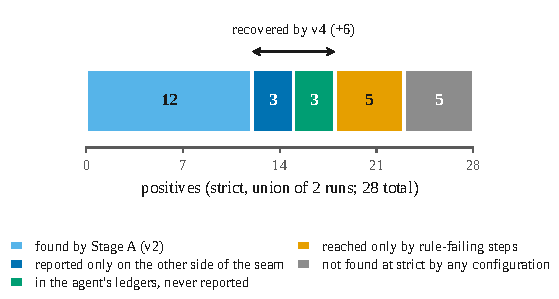
\includegraphics[width=\columnwidth]{fig-loss.pdf}
\caption{Anatomy of strict recall on dev-v4 (union of 2 runs, measured).
Each recovered hit is traced to the judge-accepted warning and the no-drop
candidate or multi-location sibling that produced it. ``v4 kept'' denotes v4.}
\label{fig:loss}
\end{figure}

\para{Anatomy of the gain}
Figure~\ref{fig:loss} partitions the 28 flaws. Stage~A finds 12. Each of the
6 recovered flaws was already in the agent's working state. \emph{Placement
(3)}: Stage~A reported the root cause, but on the other side of the seam; the
hit comes from a row no-drop restored at the auditor's location or from a
multi-location sibling. \emph{Never reported (3)}: the value sat in an
unbound row, an unconstrained statement row or a withdrawn draft, dismissed
once because the consuming contract ``is not in the repository'' and once
because the value at stake seemed too small. Across all 82 Stage~A runs the agent left
427 recorded suspicions without a final warning of their own (239 unbound
effect rows, 146 unconstrained statement rows, 42 withdrawn drafts), about 5
per run. No-drop found an admissible reason to drop 317. It restored 110,
merged into 72 warnings, 0.9 per run; by keyword coding of its stated
reasons, roughly 80 had been reported only at another location and 30 not at
all.

\para{Case study: a zkVM light client}
A light-client contract accepts a zkVM receipt and stores new headers, state
roots and the next sync committee. The guest reads the whole starting store
from private input and commits only a hash of the starting committee.
Stage~A's statement ledger recorded \emph{prevHeader: constrained: no; read
from program input, never compared to a public input}, yet its final answer
reported the problem only at the contract's \texttt{update}; the auditor
located it in the guest. No-drop dropped six candidates as covered and two
as harmless, but restored three statement rows, because their primary
location, the guest's \texttt{main}, differs from the warning's.
Multi-location then linked guest and contract under one finding. The item
went from 0 to 2 strict hits, both from tool-less calls.

\para{More knowledge, more looking, less specificity}
Three of the four extensions raised recall, and all four failed the rule
(Table~\ref{tab:dev}, Figure~\ref{fig:tradeoff}). \emph{Knowledge} alone
raises strict recall from 12 to 16 and makes hits more stable (mean 15.0),
but on top of v4 the union stays at 18: it finds earlier what no-drop
recovers later, and it adds Stage~A findings on patched and hard-negative
code well above run-to-run noise. \emph{Challenge} buys two flaws for about
5.5 new findings per run on those snapshots, \emph{probes} one for 13, and
\emph{inventory} none. These findings recur in both runs on the same
snapshots, so they reflect what the steps look for, not noise; whether some
are real issues outside the label set we cannot say without triage, so the
rule counts them all. A catalogue teaches the agent to \emph{suspect} more;
no-drop stops it \emph{losing} what it already suspects, which is cheaper and
far more specific. Pursuing recall without the rule would have reached 20 of
28 at 7.93 new findings per 10 and twice the volume.

\begin{figure}[t]
\centering
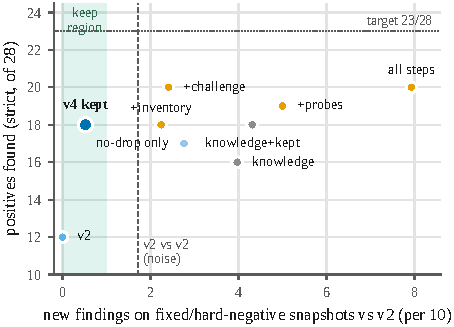
\includegraphics[width=\columnwidth]{fig-tradeoff.pdf}
\caption{Strict recall against new findings on fixed and hard-negative
snapshots, relative to v2 (dev-v4, measured). The shaded band is the keep
rule's tolerance; the dashed line is v2 against itself. Only v4 lies inside
the band. The dotted line is the 80\% target set before the build. ``v4 kept'' denotes v4.}
\label{fig:tradeoff}
\end{figure}

\begin{table}[t]
\centering
\caption{Strict union recall on dev-v4 by pattern (measured).}
\label{tab:pattern}
\footnotesize
\begin{tabular}{@{}lrrrr@{}}
\toprule
\textbf{Pattern} & \textbf{Flaws} & \textbf{v2} & \textbf{v4} & \textbf{All steps} \\
\midrule
P1 effect & 8 & 5 & 7 & 7 \\
P2 context & 10 & 4 & 6 & 8 \\
P3 replay & 3 & 2 & 3 & 2 \\
P4 verifier & 3 & 1 & 2 & 2 \\
P5 interface & 3 & 0 & 0 & 1 \\
other & 1 & 0 & 0 & 0 \\
\bottomrule
\end{tabular}
\end{table}

\para{What remains}
Five flaws are found by no configuration: a parser differential between the
signed and the parsed region of an e-mail, a library getter that skips its
sibling's anchor check, a chain identifier that stays a prover input, a
verifier chosen from a class anyone can register, and a batch check that does
not tie each (image, journal) claim to its request. Each requires following
the value into a library, a registry or an aggregation helper that the
consumer function does not show. Five more are reached only by rejected
steps. By pattern (Table~\ref{tab:pattern}), gains concentrate in P1 and P2;
interface mismatches (P5) remain unsolved, 0 of 3. Stability is also a limit (Figure~\ref{fig:items}): 8 of v4's 18 hits are
fragile, so a single run finds about 14 and a second adds about 4
(Appendix~\ref{app:items}). Knowledge makes hits more stable (3 fragile)
but not broader.

\begin{figure*}[t]
\centering
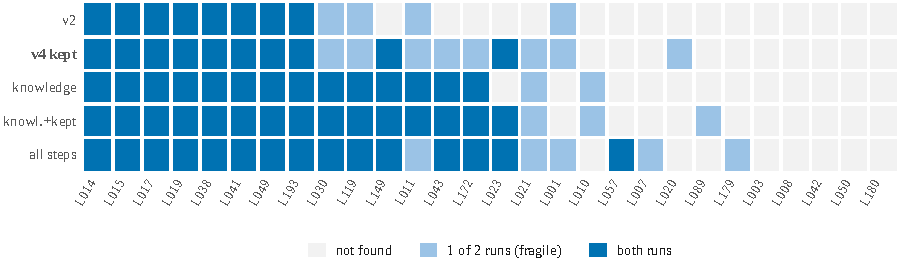
\includegraphics[width=\textwidth]{fig-items.pdf}
\caption{Strict outcome per dev-v4 flaw (columns) and configuration (rows) over
two runs, sorted by total hits (measured). ``v4 kept'' denotes v4.}
\label{fig:items}
\end{figure*}

\finding{The agent's recoverable misses were not unseen: it reported them on
the wrong side of the proof boundary or recorded them and let them go. One
tool-less re-adjudication under closed rules recovers them (12$\to$18 of
28 over two runs, 10.0$\to$14.0 per run, $p=0.031$) with no strict false finding on patched code, while knowledge
and extra tool-using looks buy recall only with false findings.}

\subsection{RQ4: Held-out data}\label{sec:eval-heldout}

\begin{table}[t]
\centering
\caption{\DEMO{Frozen v4 on held-out data: strict hits, median of three runs
(min--max).} v2's single pre-amendment run on the check set found 2 of 7
(measured). Fresh audited = check set + round~3.}
\label{tab:final}
\footnotesize
\setlength{\tabcolsep}{3pt}
\begin{tabular}{@{}lccc@{}}
\toprule
\textbf{Set (positives)} & \textbf{v2} & \textbf{Plain LLM} & \textbf{v4} \\
\midrule
Check set (7) & \DEMO{2 (2--3)} & \DEMO{2 (1--2)} & \DEMO{3 (3--4)} \\
Round~3 (7) & \DEMO{2 (1--2)} & \DEMO{1 (1--2)} & \DEMO{3 (2--4)} \\
\textbf{Fresh audited (14)} & \DEMO{4 (3--5)} & \DEMO{3 (2--4)} & \DEMO{\textbf{6} (5--7)} \\
\quad union of 3 runs & \DEMO{5} & \DEMO{4} & \DEMO{8} \\
\quad mechanism level & \DEMO{6} & \DEMO{5} & \DEMO{8} \\
B3 mutants (37) & \DEMO{21 (20--23)} & \DEMO{11 (9--12)} & \DEMO{\textbf{27} (25--29)} \\
\quad proof side (11) & \DEMO{3} & \DEMO{1} & \DEMO{6} \\
\midrule
Decoys flagged (5) & \DEMO{0} & \DEMO{2} & \DEMO{1} \\
Hard negatives flagged (3) & \DEMO{0} & \DEMO{0} & \DEMO{1} \\
\bottomrule
\end{tabular}
\end{table}

\DEMO{v4 was frozen, and its tag and file hashes appended to the
pre-registration, before it ran on any held-out set. On the 14 fresh audited
flaws it finds a median of 6 (43\%, 95\% CI 21--67\%) against 4 for v2 and 3
for the plain LLM (Table~\ref{tab:final}); over three runs it finds 8. On B3
it finds 27 of 37 mutants (73\%) against 21 and 11, and 6 of the 11
proof-side ones against 3. v2 and v4 ran independently, so v4 can lose hits;
counting a flaw as found when a tool finds it in at least two of its three
runs, v4 gains 10 and loses 2 against v2 over all 51 held-out flaws (exact
McNemar $p=0.04$); 8 of the 10 gains come from
restored or sibling warnings, the same mechanism as on dev. It flags one of
five decoys and one of three hard negatives, and no fixed twin at strict.
The held-out gain is smaller than the dev gain, as expected for a method
developed on dev data; the held-out audited recall (43\%) is below the
single-run dev recall (50\%).}

\begin{figure}[t]
\centering
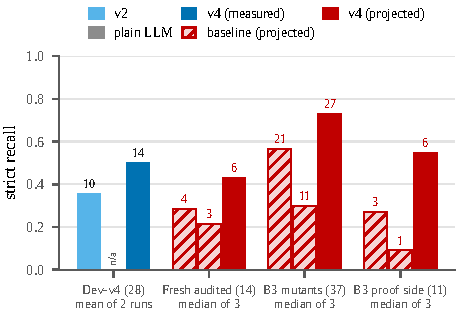
\includegraphics[width=\columnwidth]{fig-heldout.pdf}
\caption{Strict recall on dev-v4 (measured, mean of 2 runs) and on held-out
sets (\DEMO{projected, median of 3 runs}). The plain LLM was not run on
dev-v4.}
\label{fig:heldout}
\end{figure}

\finding{\DEMO{The improvement transfers: on 51 held-out flaws, v4 gains 10
and loses 2 against v2, mostly through the same placement and
non-reporting repairs. Proof-side flaws remain the hardest: v4 finds about
half.}}

\subsection{RQ5: New binding flaws}\label{sec:eval-rq5}

\DEMO{We ran frozen v4 once, as pre-registered, on the latest audited
commits of 25 ZK applications from our collection that were never used in
development or evaluation. It reported 46 findings (1.8 per application). Two
authors judged each independently from its evidence (phase~2,
Section~\ref{sec:eval-rq6}): 9 are binding flaws, of which 6 match findings
the auditors had already reported and 3 are previously unreported
(Table~\ref{tab:new}). We confirmed each new flaw with an attack test that a
second author re-ran, checked whether the current release is affected, and
reported it through the project's security contact. In N1, a
social-recovery module accepts a proof over an account's guardians but takes
the new owner set from calldata, so anyone who observes a valid recovery
proof can install its own owners.}

\begin{table}[t]
\centering
\caption{\DEMO{Previously unreported binding flaws found by \tool{}.} Evid.:
strongest executed evidence (E3 real proof, E2 mock verifier). Projects are
anonymized until disclosure completes.}
\label{tab:new}
\footnotesize
\setlength{\tabcolsep}{2.5pt}
\begin{tabular}{@{}llllll@{}}
\toprule
\textbf{ID} & \textbf{Domain} & \textbf{Pat.} & \textbf{Unbound value} & \textbf{Evid.} & \textbf{Status} \\
\midrule
\DEMO{N1} & \DEMO{social recovery} & \DEMO{P1} & \DEMO{new owner set} & \DEMO{E3} & \DEMO{fixed} \\
\DEMO{N2} & \DEMO{bridge} & \DEMO{P2} & \DEMO{source chain ID} & \DEMO{E3} & \DEMO{acknowledged} \\
\DEMO{N3} & \DEMO{token claim} & \DEMO{P3} & \DEMO{nullifier mod $r$} & \DEMO{E2} & \DEMO{no reply (40\,d)} \\
\bottomrule
\end{tabular}
\end{table}

\subsection{RQ6: Precision, evidence and cost}\label{sec:eval-rq6}

\para{Two-phase ground truth}
Audit labels bound recall but not precision: a finding that matches no label
is either false or a flaw the auditor missed. Phase~1 matches findings to
labels or mutants; phase~2 sends every unmatched finding to two authors, who
judge it independently from its evidence package with C1--C3 as the rubric,
then resolve disagreements. \DEMO{They agreed on 86\% of the 113 phase-2
findings before discussion ($\kappa=0.74$).}

\begin{table}[t]
\centering
\caption{\DEMO{Every v4 finding on the blind sets.} Corr.: matched a label or
mutant, or (hunt) judged a real binding flaw in phase~2; Pol.: real but allowed by $\Pi$; Unc.:
undecided; Test: correct / false findings with a succeeding attack test (E2
or E3); Min: median review minutes per project.}
\label{tab:evidence}
\scriptsize
\setlength{\tabcolsep}{2.4pt}
\begin{tabular}{@{}lrrrrrrrr@{}}
\toprule
\textbf{Set} & \textbf{Find.} & \textbf{Corr.} & \textbf{Pol.} & \textbf{Unc.} & \textbf{FP} & \textbf{Prec.} & \textbf{Test} & \textbf{Min} \\
\midrule
Check + round 3 & \DEMO{26} & \DEMO{6} & \DEMO{6} & \DEMO{4} & \DEMO{10} & \DEMO{23\%} & \DEMO{3 / 1} & \DEMO{14} \\
B3 mutants & \DEMO{74} & \DEMO{27} & \DEMO{9} & \DEMO{7} & \DEMO{31} & \DEMO{36\%} & \DEMO{18 / 2} & \DEMO{7} \\
Hunt & \DEMO{46} & \DEMO{9} & \DEMO{7} & \DEMO{5} & \DEMO{25} & \DEMO{20\%} & \DEMO{6 / 1} & \DEMO{24} \\
\midrule
Total & \DEMO{146} & \DEMO{42} & \DEMO{22} & \DEMO{16} & \DEMO{66} & \DEMO{29\%} & \DEMO{27 / 4} & \\
\bottomrule
\end{tabular}
\end{table}

\para{Precision}
\DEMO{Of v4's 146 findings on the blind sets, 42 are correct (29\%, 95\% CI
22--37\%) and 22 more describe real caller-chosen values that the intended
policy allows (Table~\ref{tab:evidence}); phase~2 found no unlabeled binding
flaw on the audited or mutant sets. Precision depends on the target: 36\% on
mutants, 23\% on audited code and 20\% in the hunt, where the code has
already passed an audit and most findings concern paths the audit covered.
An auditor reads about two findings per project, each with its proof-side and
consumer-side locations.}

\para{Executable evidence}
\DEMO{After we made the scaffold derive its EVM version from the sources (a
fixed target had failed on a vendored library that uses a newer opcode), 7 of
v4's 18 dev hits reached E2 and 3 reached E3, with no E2 or E3 on the 29
fixed or hard-negative snapshots, which satisfies part (iii) of the keep
rule. On the blind sets, 27 of the 42 correct findings carry a succeeding
test, against 4 of the 66 false ones. A finding with a passing test took a
median of 6 minutes to review, one without 15 (6 against 11 within B3, where
mutants are alike); this is an association, not a controlled effect.}

\para{Cost}
On dev-v4, Stage~A takes a median of 244\,s (76--615\,s) and \$0.84
(\$0.19--2.90) per scan, scaling with repository size
(Appendix~\ref{app:extra}); the post-stage adds 29\,s and \$0.15. The loop
adds a median of \$0.39 (at most \$2.40) on development targets, 80\% of it
for drafting scaffolds; template attempts cost nothing. \DEMO{On the
held-out sets a full scan costs a median of \$1.46 and 6.2 minutes.} The
analyzers run in minutes but only after a human has made each project build,
and the assisted fuzzer needs 5--45 minutes of expert wiring per target.

\finding{\DEMO{About three findings in ten are real binding flaws and two
more in ten are policy-allowed; a passing attack test separates them well
(27 of 42 correct, 4 of 66 false). A scan costs about \$1.50.}}

\section{Discussion}\label{sec:discussion}

\para{Beyond binding}
We expect the no-drop idea to transfer to any LLM auditor that keeps
intermediate notes: a withdrawn or relocated suspicion deserves at least as
much scrutiny as the suspicion itself, and structured intermediate output is
what makes ``never seen'' and ``seen and lost'' distinguishable when the
agent is evaluated.

\para{Lessons for developers}
The signature analogy doubles as a checklist. \emph{Sign what you act on}:
every recipient, amount and fee is a public input or hashed into one that the
consumer recomputes (P1). \emph{Separate domains}: commit to chain, contract
and policy, and check roots and prior states against the consumer's own
storage (P2). \emph{Derive nonces from the statement} and reduce them into the
field before storing (P3). \emph{Pin the key} and check the verifier's result
(P4). \emph{Test with a malicious caller}: an honest proof submitted by a
second account with changed arguments must fail. This single test, the
invariant of Section~\ref{sec:design-loop}, is what turned the fuzzer from 0
to 5 of 13 flaws.

\para{Toward binding by construction}
Binding flaws exist because the public-input vector is an untyped array whose
meaning is restated by hand in the circuit, the verifier wrapper and the
consumer. Circuit languages could export a \emph{typed statement} schema from
which verifier generators emit a typed consumer interface, removing P5 and
making P1 visible. A standard \emph{effect commitment} over recipient,
amount, chain, contract and nonce, computed in the circuit and recomputed in
the consumer, would play the role EIP-712~\cite{eip712} plays for signatures
and address P1--P3 together. Verifier libraries could make the key or program
ID an immutable constructor argument (P4). \DEMO{Applied to the 87 core
findings, typed statements would have prevented 41\% and effect commitments
63\%.} The binding question---does the verified object commit to every value
the effect uses?---also applies beyond ZK: to signed permits that omit the
spender, TEE attestations whose report data omits the request, and bridge
messages that omit the destination domain.

\subsection{Threats to validity}\label{sec:threats}

\para{Selection and labels}
We study public audits of projects that chose to publish them; unaudited
projects may differ. Labels were proposed by an LLM and adjudicated by two
raters who discussed every item, so they are not independent annotations; a
written guide, a code-level pass for every evaluated item \DEMO{and a blind
relabel ($\kappa=0.78$)} mitigate this, and we release every label with its
notes. Auditors' locations are one of several valid ones; mechanism-level
recall bounds the effect.

\para{Development bias}
The post-stage rules were written while studying dev misses, and one
admissibility rule and one catalogue fact were informed by an item in the
original check split, which is among the gains; dev recall is therefore
optimistic, and we report it only as development evidence. The keep rule was
fixed after a preliminary single-run measurement of no-drop and
multi-location and before any other step was measured; one counting detail
was corrected afterwards, which turned the knowledge step from pass to fail
and changed no other decision (Appendix~\ref{app:count}). Held-out claims
rest on sets the building process never saw.

\para{Location credit and judge}
Multi-location reporting raises the chance of matching the auditor's
location. The judge's mechanism check, 0 of 17 fixed twins flagged at
strict, and per-finding counting bound this effect but do not remove it. The
judge is an LLM with a frozen prompt and about 5\% verdict instability; all
configurations share cached verdicts.

\para{Variance and contamination}
With 28 dev flaws and two runs, intervals are wide and 8 of 18 hits fragile;
held-out numbers are medians of three runs. Audit reports may be in the
model's training data. Mutants are new code, snapshots contain no audit text,
and fixed twins are a partial control: a model recalling a report would also
flag the patched code, and v4 flags none at strict. \DEMO{On round~3, whose
reports were all published after the model's training cutoff, v4 finds 3 of 7,
as on the check set, and the three new flaws were unknown before our scans.}

\para{Leakage}
The coordinating author saw v2's test results, so B1 is development data for
v4. Every version was built by a separate process restricted to development
data, test benchmarks live in a separate repository, and every exposure is
logged (Appendix~\ref{app:timeline}).

\subsection{Limitations}\label{sec:limits}
\tool{} needs an LLM and costs about one to two dollars per scan, and all
runs use one model. Its helpers are syntactic, so library code that is not
vendored is a blind spot, and the residue of RQ3 sits exactly there. The
loop targets EVM consumers: flaws whose effect lies in a zkVM host or off
chain stay at E1, and real-proof tests need proving artifacts that most
projects do not ship. Binding is relative to the intended policy $\Pi$, which
\tool{} infers from code and documentation and can get wrong.

\section{Related Work}\label{sec:related}

\para{ZK vulnerability studies}
Chaliasos et al.\ classify 141 vulnerabilities in SNARK systems by layer
(circuit, front end, back end, integration)~\cite{sok-snark-bugs}. Their
integration layer holds 13 bugs, 9 of them public inputs the application
does not check, and they report that no defense targets this layer. Other
studies and trackers catalog circuit and auditing
flaws~\cite{zkp-vuln-audit,zk-bug-tracker,zkbugs} and zkVM
vulnerabilities~\cite{zkvm-study}. Individual binding flaws therefore appear
in this literature: the tracker documents an airdrop whose nullifier aliases
modulo $r$ (our P3) and describes how a proof can be replayed with a changed
public input that the compiler optimized out of the circuit (our
P1)~\cite{zk-bug-tracker}.
These works catalog flaws by layer or root cause, one instance at a time; we
define the class by the cross-layer property it violates and measure it on
87 core findings.

\para{Circuit, compiler and zkVM analysis}
Most ZK tools check the relation $R$. circomspect~\cite{circomspect} lints
Circom, Ecne~\cite{ecne} and Picus~\cite{picus} decide whether a circuit
uniquely determines its outputs, ZKAP~\cite{zkap} queries a circuit
dependence graph for anti-patterns, CIVER~\cite{civer} and
Coda~\cite{coda} verify circuit specifications, and zkFuzz~\cite{zkfuzz}
fuzzes circuits for under- and over-constraints. Circuzz and
MTZK~\cite{circuzz,mtzk} test circuit compilers, and Arguzz, Beak and a
miscompilation study~\cite{arguzz,beak,zkvm-miscompile} target zkVMs. Their detection rate drops from 45.7\% on isolated targets to 19.6\% on
full codebases, and practitioners name integration as a major
gap~\cite{zk-tools-sok}.
A binding flaw can exist under a fully constrained, correctly compiled
circuit, because it concerns which consumer values the statement was meant
to fix. \tool{} analyzes the circuit and the consumer together.

\para{Smart-contract analysis}
Static analyzers~\cite{slither,securify}, symbolic
executors~\cite{mythril,manticore} and fuzzers~\cite{echidna,ityfuzz,foundry}
miss most annotated~\cite{smartbugs} and contest-exploitable~\cite{exploitable-bugs}
vulnerabilities. Invariant inference~\cite{smartinv},
LLM-generated properties~\cite{propertygpt} and signature-replay
detection~\cite{lasir} supply some missing specifications, but none has a
notion of a proved statement, so an unbound recipient looks like an ordinary
parameter.

\para{LLM-based auditing}
GPTScan~\cite{gptscan}, LLM4Vuln~\cite{llm4vuln} and iAudit~\cite{iaudit}
combine LLMs with analysis or fine-tuned agents, and A1, ReX and
PoCo~\cite{a1-agent,rex,poco} validate exploits by execution. \tool{} shares
the execution loop, but its procedure is derived from a precise definition
and forces checkable ledgers over two artifacts. Studies of LLM auditors
measure what they report; the ledgers let us measure what they \emph{knew}
and discarded, and show that for a strong agent the recoverable misses come
from placement and non-reporting rather than ignorance.

\para{Binding in cryptography and protocols}
Signatures of knowledge~\cite{sig-of-knowledge,snarky-sigs} bind a proof to a
message, and simulation extractability prevents mauling a proof into one for
a new statement. Groth16~\cite{groth16} proofs are re-randomizable yet
statement non-malleable~\cite{groth16-randomization}, which is why
$\mathsf{keccak}(\pi)$ fails as a replay key (P3). Weak
Fiat--Shamir~\cite{weak-fs} breaks soundness, and Portal~\cite{portal} fixes
proof replay at identity contracts. These results protect the statement; a
binding flaw concerns a value that was never in it. Our patterns mirror
cryptographic API misuse~\cite{egele-crypto-misuse,cryptoguard,crysl,cognicrypt}
and signed-token flaws such as a relying party using an email the signature
does not cover~\cite{sso-flaws}. EIP-712~\cite{eip712} adds domain separation
to signed messages, front-running~\cite{flashboys} turns an unbound recipient
into theft, and bridges fail the same way for verified
messages~\cite{bridge-sok,xscope,smartaxe,interop-sok}. To our knowledge we
are the first to define statement-to-effect binding for ZK consumers as a
property, measure its prevalence across audits, and detect it
automatically.

\section{Conclusion}\label{sec:conclusion}

A valid proof certifies a statement, not an effect. We defined binding as the
requirement that every value deciding an effect follows from the statement or
is left open by the intended policy, classified its violations into five
patterns that mirror signature misuse, and found 87 core instances in public
audits, 78\% of the rated ones Critical or High. No circuit or contract
analyzer sees them, because the specification lives between the two.
\tool{} reconstructs it as two ledgers, and those ledgers show that a strong
agent's recoverable misses are flaws it found and then misplaced or let go.
Keeping them costs one tool-less call and raised dev recall from 12 to 18 of
28 over two runs (10.0 to 14.0 per run) with no strict false finding on
patched code. \DEMO{The gain held on 51
held-out flaws and uncovered three new ones.} Binding should be checked as
routinely as a signature.

\section*{Ethics Considerations}
This work uses public audit reports and public source code. Every attack test
runs on a local chain with synthetic assets; no transaction was sent to any
public network, and the released loop has no network access by design.
\tool{} is dual-use, but binding flaws are already found by auditors and
attackers reading contracts; the asymmetry it reduces is between well-funded
audits and the many projects that cannot afford one. \DEMO{We reported the
three new flaws of Section~\ref{sec:eval-rq5} privately through each
project's security contact with a 90-day window; Table~\ref{tab:new} gives
their status, and their details are withheld until disclosure ends.} No human
subjects were involved.

\section*{Open Science}
\DEMO{The artifact (\url{https://anonymous.4open.science/r/bindcheck}) contains
the dataset (labels, guide and the script that rebuilds every cleaned
snapshot from public commits), benchmarks B1--B3 with ground truth, the
\tool{} source and frozen configuration, the matching rules and judge prompt
with all cached verdicts, every run transcript and output with run dates,
and the scripts behind every table and figure.}

\bibliographystyle{IEEEtran}
\bibliography{refs}
\appendices
\section{Labeling Guide Summary}\label{app:labels}
For each candidate, raters recorded:
\begin{itemize}
\item binding (Y/N/U);
\item whether the issue is a proof-system soundness bug;
\item the pattern (P1--P5, OTHER or NA);
\item C1--C3 individually (met, fails, unclear);
\item the effect, the unbound value and the intended policy (FULL tier);
\item confidence and notes.
\end{itemize}
The exclusions of Section~\ref{sec:definition} and the hard cases (attested
verification, signatures instead of proofs, multi-issue findings) follow the
guide in the artifact.

\section{No-Drop Admissibility Rules}\label{app:nodrop}
A candidate (withdrawn draft, unbound effect row, unconstrained statement row)
may be dropped \textbf{only} if: (1)~a final warning already reports the same
unbound value at the same primary location (file and function); (2)~the
review cited a concrete check (file:line) that binds the value on every path,
or showed that the attack only makes verification fail; (3)~a numbered
exclusion genuinely applies (quoted); or (4)~there is no concrete attacker
action (nothing the attacker changes while keeping a valid proof). Every other
reason is inadmissible, in particular: the consumer is not in the repository
(report at the circuit, guest or library); the attack needs another flaw as
well; the issue was folded into a finding whose primary location differs; it
is ``secondary'' to a bigger issue; it could not be traced to an effect
function although the proving component leaves a value the consumer acts on
unconstrained. Restored warnings use only paths and functions present in the
material, one per root cause, at the definition rather than per instantiated
copy.

\section{Scoring, Judge and Keep-Rule Counting}\label{app:count}
\para{Matching}
Strict: the warning's own file (basename) and function equal the ground-truth
location, case-insensitively and ignoring qualifiers, and the judge confirms
the mechanism. Loose: location only. Mechanism: any warning in the snapshot
that the judge accepts. A v1.1 amendment, adopted after round~1 and applied to
all tools, added the case-insensitive matcher and the mechanism level.

\para{Judge}
For each flaw the judge receives the ground-truth unbound value and effect
and, per candidate warning in the same snapshot, its pattern, effect,
unbound value and explanation, and answers yes or no. The prompt is frozen
(identified by its hash), the call has no tools, verdicts are cached per
(warning, flaw) pair, and a failed or non-binary answer aborts scoring rather
than counting as no.

\para{Keep rule}
For each configuration and run we count (a)~on every fixed-twin snapshot,
every \texttt{finding\_id} group whose locations are disjoint from all
locations the comparison configuration reports there, and (b)~every hard
negative flagged by the configuration but not by the comparison. The count is
averaged over the two runs and normalized per 10 of the 29 snapshots that
hold a fixed twin or hard negative; normalizing per unit (45) changes no
decision. Run-to-run noise is the same count between two runs of one
configuration. \emph{Correction after results:} for steps that change
Stage~A itself (knowledge), (a) had excluded new Stage~A findings and
undercounted; counting them raised knowledge from 0.52 to 3.97 per 10 and
turned a pass into a fail. No other decision changed.

\section{Execution-Loop Guards}\label{app:guards}
The first loop version produced a false pass: a scaffold deployed the
contract from the honest account, which made it the owner, and the owner's
repeated call to an owner-only mint looked like a replay. Six guards close
such loopholes. (O1)~Before a replay or same-sender success counts, the
honest call is retried from a fresh account; if access control rejects it,
the success is void. (O2)~Scaffolds deploy and grant roles from a separate
administrator. (O3)~A replay success requires a replay-key row, and the
second effect must touch that key. (O4)~A scaffold whose honest run fails a
check is redrafted. (O5)~The agent cannot give up before an LLM attempt, and
a give-up must cite an earlier outcome. (O6)~A mock verifier cannot tell
verifiers apart, so a success that swaps the verifier, proof type or key
counts only on the real verifier. Under a selection rule fixed in advance we
also compared discovery variants: an extractor-based coverage check found 70
rows the ledgers missed and judged none unbound, an execution sweep attacked
60 of 645 effect rows without success, and a depth pass into vendored
dependencies added one strict hit within run-to-run variance at 2.4 times the
cost. More reading did not help; the misses were judgments.

\section{Per-Item Results on Dev-v4}\label{app:items}
\begin{table*}[!htb]
\centering\footnotesize
\caption{Strict hits out of 2 runs per dev-v4 flaw. Layer: S Solidity, C
circuit, R Rust zkVM. ND: no-drop only; K: Stage A with knowledge; All: all
post steps. Recovery: how v4 obtains the hit.}
\setlength{\tabcolsep}{2.6pt}
\begin{tabular}{@{}llllrrrrrrl@{}}
\toprule
Item & Split & L & Pat. & v2 & ND & v4 & K & K+v4 & All & Recovery\\
\midrule
L001 & old-check & C & P2 & 1 & 1 & 1 & 0 & 0 & 1 & Stage A \\
L003 & old-tune & R & other & 0 & 0 & 0 & 0 & 0 & 0 & -- \\
L007 & v4-tune & S & P5 & 0 & 0 & 0 & 0 & 0 & 1 & -- \\
L008 & old-tune & R & P2 & 0 & 0 & 0 & 0 & 0 & 0 & -- \\
L010 & v4-tune & S & P1 & 0 & 0 & 0 & 1 & 1 & 0 & -- \\
L011 & old-tune & S & P1 & 1 & 1 & 1 & 2 & 2 & 1 & Stage A \\
L014 & old-tune & S & P2 & 2 & 2 & 2 & 2 & 2 & 2 & Stage A \\
L015 & v4-tune & S & P1 & 2 & 2 & 2 & 2 & 2 & 2 & Stage A \\
L017 & old-check & S & P1 & 2 & 2 & 2 & 2 & 2 & 2 & Stage A \\
L019 & old-check & S & P4 & 2 & 2 & 2 & 2 & 2 & 2 & Stage A \\
L020 & v4-tune & S & P3 & 0 & 0 & 1 & 0 & 0 & 0 & multi-loc.\ (placement) \\
L021 & v4-tune & S & P4 & 0 & 1 & 1 & 1 & 1 & 1 & no-drop (never reported) \\
L023 & old-check & S & P1 & 0 & 2 & 2 & 0 & 2 & 2 & no-drop (placement) \\
L030 & old-tune & R & P2 & 1 & 1 & 1 & 2 & 2 & 2 & Stage A \\
L038 & old-tune & C & P3 & 2 & 2 & 2 & 2 & 2 & 2 & Stage A \\
L041 & old-check & S & P1 & 2 & 2 & 2 & 2 & 2 & 2 & Stage A \\
L042 & v4-tune & S & P4 & 0 & 0 & 0 & 0 & 0 & 0 & -- \\
L043 & v4-tune & C & P1 & 0 & 1 & 1 & 2 & 2 & 2 & no-drop (never reported) \\
L049 & old-check & S & P3 & 2 & 2 & 2 & 2 & 2 & 2 & Stage A \\
L050 & old-tune & S & P2 & 0 & 0 & 0 & 0 & 0 & 0 & -- \\
L057 & v4-tune & S & P2 & 0 & 0 & 0 & 0 & 0 & 2 & -- \\
L089 & v4-tune & S & P5 & 0 & 0 & 0 & 0 & 1 & 0 & -- \\
L119 & v4-tune & R & P2 & 1 & 1 & 1 & 2 & 2 & 2 & Stage A \\
L149 & v4-tune & R & P2 & 0 & 1 & 2 & 2 & 2 & 2 & no-drop / multi-loc.\ (placement) \\
L172 & v4-tune & R & P2 & 0 & 1 & 1 & 2 & 2 & 2 & no-drop (never reported) \\
L179 & v4-tune & R & P2 & 0 & 0 & 0 & 0 & 0 & 1 & -- \\
L180 & v4-tune & S & P5 & 0 & 0 & 0 & 0 & 0 & 0 & -- \\
L193 & v4-tune & S & P1 & 2 & 2 & 2 & 2 & 2 & 2 & Stage A \\
\midrule
\multicolumn{4}{@{}l}{By layer (strict union): S (18) / C (3) / R (7)} & 8/2/2 & & 11/3/4 & & 12/2/4 & 12/3/5 & \\
\bottomrule
\end{tabular}
\end{table*}

\section{What the Builders Saw}\label{app:timeline}
Table~\ref{tab:timeline} lists, for each version, which data had been seen
before its freeze. ``Builder'' is the separate tool-building process, which
could read only development data; ``author'' is the coordinating author;
``lane'' is any other automated process. Every exposure, including
metadata-only touches, is logged in the artifact.

\begin{table}[!htb]
\centering
\caption{Exposure timeline (2026, all dates in November unless noted).}
\label{tab:timeline}
\scriptsize
\setlength{\tabcolsep}{2pt}
\begin{tabular}{@{}lp{3.0cm}p{3.5cm}@{}}
\toprule
\textbf{Date} & \textbf{Event} & \textbf{Seen, and consequence} \\
\midrule
22 & Audit sweep & author: titles of 3 reserved families' pages (metadata only) \\
24 & Labels frozen; family split & author: code evidence of 3 items $\Rightarrow$ their families forced to dev before the split \\
24 & v1 and plain LLM on round~1 & author: round-1 GT and per-item warnings $\Rightarrow$ v2 built by a fresh lane from dev only \\
24 & v2 frozen; run on rounds 1--2, B2 & author: round-2 labels while v2 was being built (never sent to the builder) \\
25 & B3 frozen; v3 launched & builder: one test-derived phrase in a brief for under a minute, then retracted $\Rightarrow$ v3 reruns on B1/B2 not blind \\
25 & Characterization (§4) & lane: report text of all 103 binding labels, incl.\ test, for D3/D4 tags; no code, no tool work \\
26 & v3 frozen; pre-registration & builder: dev only \\
26 & Amendment A1 & author: v2 per-item results, incl.\ the check set; B1 families released to dev; check set (seed 20261126) withheld from the builder \\
26--28 & v4 built on dev-v4 & builder: dev-v4 (28 flaws); never the check set, B3, round~3 \\
\DEMO{29} & \DEMO{v4 frozen; round-3 list appended} & \DEMO{author: round-3 labels} \\
\DEMO{30--Dec 2} & \DEMO{v4 on check set (once), B3, round~3, hunt} & \DEMO{builder: none of them} \\
\bottomrule
\end{tabular}
\end{table}

\section{Benchmark Coverage}\label{app:coverage}
\begin{table}[h]
\centering
\caption{What each benchmark covers. Layers count positives by the location
of the flaw.}
\label{tab:coverage}
\scriptsize
\setlength{\tabcolsep}{2pt}
\begin{tabular}{@{}lrrp{3.6cm}@{}}
\toprule
\textbf{Benchmark} & \textbf{Pos.} & \textbf{Hosts} & \textbf{Layers (Solidity / circuit / Rust guest or host)} \\
\midrule
B1 (rounds 1--2) & 22 & 13 fam. & 15 / 2 / 5 \\
B2 mutants & 27 & 3 small & 23 / 4 / 0 \\
Check set (from B1) & 7 & 7 fam. & 5 / 1 / 1 \\
Round~3 & \DEMO{7} & \DEMO{5 fam.} & \DEMO{3 / 1 / 3} \\
B3 mutants & 37 & 5 apps & 26 / 9 / 2 \\
\bottomrule
\end{tabular}
\end{table}

\section{One Finding End to End}\label{app:trace}
We trace the proof-marketplace flaw of Figure~\ref{fig:motivating}
through the artifact.
\begin{enumerate}
\item \emph{Audit report.} Veridise, April 2025, finding V-BML-VUL-001:
fulfillment does not validate request identifiers.
\item \emph{Label.} Item L193 in \texttt{LABELS-v1.csv}: binding Y, P1,
C1--C3 met, family RISC Zero/Boundless, test split, round~2.
\item \emph{Ground truth.} Row L193 in the round-2 location file:
\texttt{BoundlessMarket.sol}, function \texttt{\_fulfillAndPay}; unbound value
\texttt{Fulfillment.id}.
\item \emph{Warning.} Warning 1 of \texttt{tool-v2/L193/vuln.json}, at
the same function, naming the calldata identifier and the journal digest.
\item \emph{Score.} Strict, loose and mechanism-level hit; the judge prompt
hash and verdict are in the scoring log, and the fixed version raises no
warning.
\end{enumerate}

\section{Additional Figures and Tables}\label{app:extra}

\begin{figure}[!htb]
\begin{lstlisting}[mathescape]
Scan(target):
  copy target read-only; I := Inventory(copy)       // E_i, S_j
  L_E := Agent(effect, I)                           // effect ledger
  for r in 1..2: U := I.E \ entries(L_E)
      if U = {}: break;  L_E += Agent(reprompt, U)
  L_S := Agent(statement, I, L_E)                   // statement ledger
  for r in 1..2: U := I.S \ values(L_S)
      if U = {}: break;  L_S += Agent(reprompt, U)
  W := Agent(follow, L_E, L_S)   // playbooks P1-P5, libraries
  if cost < SOFT: W += Agent(attacker, W)
  W_f := Agent(final, W)          // drop C1-C3 failures
  W_f += NoDrop(W \ W_f, unbound(L_E), open(L_S), tail)  // tool-less
  W_f += MultiLoc(W_f)            // siblings share finding_id
  for k in 0..3, u in unbound rows not settled:  // breadth-first
      t := (k = 0) ? Template(u) : Agent(attack, u, trace(u))
      trace(u) += (t, Sandbox(t))  // oracle computes outcome
  return [(w, trace(w)) for w in W_f]   // evidence package
\end{lstlisting}
\caption{The \tool{} v4 controller. Every agent step returns structured rows
that the controller checks against the inventory before it continues.}
\label{fig:controller}
\end{figure}

\begin{table}[!htb]
\centering
\caption{Detection of injected binding mutants (B2) by pattern
(strict hits / mutants). ``uns.'' = the tool cannot analyze the layer or
the run failed.}
\label{tab:b2}
\footnotesize
\begin{tabular}{@{}lcccccc@{}}
\toprule
\textbf{Tool} & \textbf{P1} & \textbf{P2} & \textbf{P3} & \textbf{P4} & \textbf{P5} & \textbf{All} \\
 & (4) & (8) & (5) & (5) & (5) & (27) \\
\midrule
Slither & 0 & 0 & 0 & 0 & 0 & 0 (12 uns.) \\
Mythril & 0 & 0 & 0 & 0 & 0 & 0 (4 uns.) \\
circomspect & -- & 1$^*$ & -- & -- & -- & 1 \\
Picus & -- & 0 & -- & -- & -- & 0 \\
\tool{} & 4 & 8 & 4 & 2 & 4 & 22 \\
\bottomrule
\multicolumn{7}{@{}l}{\scriptsize $^*$a style warning (\texttt{<--}) at the edited line, not a binding diagnosis.}
\end{tabular}
% src: benchmarks/binding-mutants-v2/RESULTS-static.md
\end{table}


\begin{figure}[!htb]
\centering
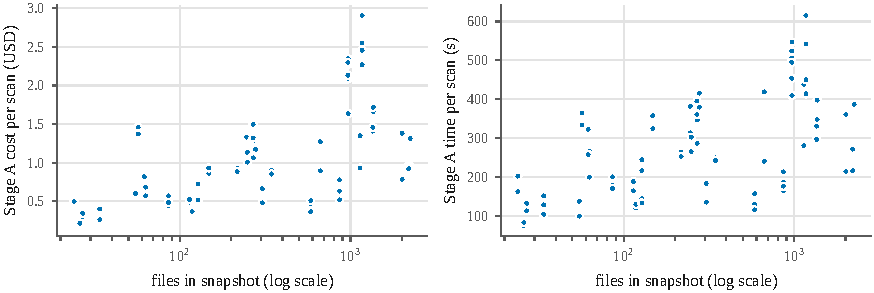
\includegraphics[width=\columnwidth]{fig-cost.pdf}
\caption{Stage A cost and time per scan against the number of files in the
snapshot (82 dev-v4 runs, measured).}
\label{fig:cost}
\end{figure}

\end{document}
